\documentclass{article}
\usepackage[utf8]{inputenc}
\usepackage{booktabs}
\usepackage{amsmath}
\usepackage{amsfonts}
\usepackage{hyperref}
\usepackage{longtable}
\usepackage{cleveref}
\usepackage{graphicx}
\usepackage{geometry}
\geometry{a4paper, margin=1in}
\usepackage{svg}
\usepackage{listings}
\usepackage{xcolor}
\usepackage{enumitem}

% Define the Julia language style
\lstdefinelanguage{Julia}%
  {morekeywords={abstract,break,case,catch,const,continue,do,else,elseif,%
      end,export,false,for,function,immutable,import,importall,if,in,%
      macro,module,otherwise,quote,return,switch,true,try,type,typealias,%
      using,while},%
   sensitive=true,%
   alsoother={\$},%
   morecomment=[l]\#,%
   morecomment=[n]{\#=}{=\#},%
   morestring=[s]{"}{"},%
   morestring=[m]{'}{'},%
}[keywords,comments,strings]

% Set the style for Julia
\lstset{%
    language         = Julia,
    basicstyle       = \footnotesize,
    keywordstyle     = \color{blue},
    stringstyle      = \color{green},
    commentstyle     = \color{red},
    showstringspaces = false,
    breaklines=true,
    numbers = left,
}


\title{ELEC\_ENG COMP\_ENG 334 Fundamentals of Blockchains and Decentralization Assignment on Probability Theory and Stochastic Processes}
\author{Chiao-Wei Hsu}
\date{\today}

\begin{document}
\maketitle

The instructor will give a brief review of probability theory in class.

\section{Probability Distributions}
Fill up the following table. You may want to consult a textbook on probability theory.

\paragraph{My Answer:} 
\Cref{tab:prob_distributions} summarizes various probability distributions.
% chktex 16
\begin{table}[h!]
    \centering
    \begin{tabular}{ccccc}
        \toprule
        \toprule
        \textbf{Name of distribution} & \textbf{Possible values} & \textbf{Probability function}                      & \textbf{Expectation} & \textbf{Variance} \\
        \midrule
        Bernoulli(q)                  & \{0,1\}                  & \( p(k) = (1-q)1_{\{k=0\}} + q1_{\{k=1\}} \) & \( q \)              & \( q(1-q) \)      \\
        Geometric(q)                  & \{1,2,\ldots\}              & \( p(k) = (1-q)^{k-1}q \)                          & \( \frac{1}{q} \)    & \( \frac{1-q}{q^2} \) \\
        Binomial(n,q)                 & \{0,1,\ldots,n\}            & \( p(k) = \binom{n}{k} q^k (1-q)^{n-k} \)          & \( nq \)             & \( nq(1-q) \)     \\
        Poisson(\(\lambda\))          & \{0,1,\ldots\}              & \( p(k) = \frac{e^{-\lambda} \lambda^k}{k!} \)     & \(\lambda\)          & \(\lambda\)       \\
        Exponential(\(\lambda\))      & \( (0,\infty) \)         & \( f(x) = \lambda e^{-\lambda x} \)                & \( \frac{1}{\lambda} \) & \( \frac{1}{\lambda^2} \) \\
        \bottomrule
        \bottomrule
    \end{tabular}
    \caption{Summary of various probability distributions. Note: $1_\text{A}$ where A is an event (or condition) stands for the indicator of that event (or condition).  It is equal to 1 if that condition holds (or the event occurs) and is otherwise equal to 0.}\label{tab:prob_distributions}
\end{table}

\section{Stochastic Modeling of Mining Times}
In this question we discuss the stochastic modeling of the block arrival times of proof-of-work mining.
\begin{enumerate}[label=(\alph*)]
    \item An excellent model for the distribution of the time between two consecutive mining events is exponential. The ideal Bitcoin expects one block mined every 10 minutes on average. Write down the exponential probability density function with specific parameter(s) to model the ideal Bitcoin.
    \paragraph{My Answer:} The exponential probability density function is given by
    \[ f(x) = \lambda e^{-\lambda x}, \]
    where \( x \) is the time between two consecutive mining events, and \( \lambda \) is the rate parameter.  In the case of the ideal Bitcoin, the rate parameter is \( \lambda = 1/10 \) (since one block is mined every 10 minutes on average), so the probability density function is
    \[ f(x) = \frac{1}{10} e^{-x/10}. \]
    \item What is the standard deviation of the inter-mining time under this model? What is the ratio of the standard deviation over the mean?
    \paragraph{My Answer:} The mean of the exponential distribution is \( 1/\lambda = 10 \) minutes.  The variance of the exponential distribution is \( 1/\lambda^2 = 100 \) minutes squared.  The standard deviation is the square root of the variance, which is \( \sqrt{100} = 10 \) minutes.  The ratio of the standard deviation over the mean is \( 10/10 = 1 \).
    \item What is the mean of the time it takes to mine 10 blocks? What is the standard deviation of this time and the ratio of its standard deviation over the mean?
    \paragraph{My Answer:} The mean of the time it takes to mine 10 blocks is \( 10 \times 10 = 100 \) minutes.  The variance of the time it takes to mine 10 blocks is \( 10 \times 100 = 1000 \) minutes squared by the property of variance of the sum of independent random variables.  The standard deviation is the square root of the variance, which is \( \sqrt{1000} = 10\sqrt{10} \approx 31.62 \) minutes.  The ratio of the standard deviation over the mean is \( 31.62/100 \approx 0.3162 \).
    \item Using data from \url{https://btc.com/block}, estimate the standard deviation of the inter-block mining time.
    \paragraph{My Answer:} The standard deviation of the inter-block mining time can be estimated by calculating the standard deviation of the time between consecutive blocks mined. \Cref{tab:block_data} shows the block data and inter-block mining times from the website.
    
    \begin{table}[h!]
        \centering
        \tiny
        \begin{tabular}{ccccccc}
            \toprule
            \textbf{Height} & \textbf{Relayed By} & \textbf{Time (UTC)} & \textbf{Tx Count} & \textbf{Reward (BTC)} & \textbf{Size (KB)} & \textbf{Inter-block Time (Min)} \\
            \midrule
            839943 & F2Pool & 2024-04-19 15:59 & 2966 & 7.358 & 1577.95 & - \\
            839942 & AntPool & 2024-04-19 15:47 & 3162 & 7.160 & 1641.14 & 12.383 \\
            839941 & Foundry USA & 2024-04-19 15:42 & 2806 & 7.144 & 1649.02 & 3.517 \\
            839940 & ViaBTC & 2024-04-19 15:39 & 3074 & 7.370 & 1545.27 & 15.083 \\
            839939 & SecPool & 2024-04-19 15:24 & 2854 & 7.321 & 1844.65 & \ldots \\\
            \ldots & \ldots & \ldots & \ldots & \ldots & \ldots & \ldots \\
            \bottomrule
        \end{tabular}
        \caption{Block Data and Inter-block Mining Times}\label{tab:block_data}
    \end{table}

    The standard deviation of the inter-block mining times can be calculated using the following Python code:

    % include python code with language setting
    \begin{lstlisting}[language=Python, gobble=8]
        import pandas as pd
        block_data = pd.read_csv('block_list_2024-03-19_2024-04-19.csv')
        # Convert 'Time (UTC)' column to datetime
        block_data['Time (UTC)'] = pd.to_datetime(block_data['Time (UTC)'])
        
        # Calculate the time differences between consecutive blocks (inter-block mining times)
        block_data['Inter-block Time (Minutes)'] = block_data['Time (UTC)'].diff(-1).dt.total_seconds() / 60
        # Absolute values for time differences
        block_data['Inter-block Time (Minutes)'] = block_data['Inter-block Time (Minutes)'].abs()
        
        # Calculate the standard deviation of the inter-block times
        std_dev_inter_block_time = block_data['Inter-block Time (Minutes)'].std()
        
        print(std_dev_inter_block_time)        
    \end{lstlisting}
    , which shows a result of 9.59 minutes.
    
\end{enumerate}

\section{Simulation of Mining Processes}

Here is some reference code in Julia language:

\begin{lstlisting}[language=Julia, gobble=4]
    # generating 5 exponential(1/2) as inter-arrival times

    using Distributions
    sample = rand(Exponential(0.5),5)
    print(sample)
    #[0.021907272304307474, 0.21703943412886162, 0.08307746218558654, 0.5667115195460581, 1.4584361639686763]

    # generating arrival times vector (arrival) from previous inter-arrival times vector (intarrival)
    intarrival = [0.021907272304307474, 0.21703943412886162, 0.08307746218558654, 0.5667115195460581, 1.4584361639686763]
    size = length(intarrival)
    arrival = zeros(size)
    arrival[1] = intarrival[1]
    for i in 2:size
        arrival[i] = intarrival[i]+arrival[i-1]
    end
    print(arrival)
    # [0.021907272304307474, 0.2389467064331691, 0.3220241686187556, 0.8887356881648137, 2.34717185213349]

    # plot some arrival times coming from two processes with different color dots
    using Gadfly
    arrival_1 = [0.021907272304307474, 0.3220241686187556]
    arrival_2 = [0.2389467064331691, 0.8887356881648137, 2.34717185213349]
    yaxis_1 = zeros(length(arrival_1))
    yaxis_2 = zeros(length(arrival_2))
    p=Gadfly.plot(layer(x=arrival_1,y = yaxis_1,color=[colorant"blue"],
    Geom.point),layer(x=arrival_2,y = yaxis_2,color=[colorant"red"], Geom.point))
    display(p)
\end{lstlisting}
The above code use different parameters than this problem requires. You need to figure out what parameters are required in this problem.

% 0.5 width, put here (h)
\begin{figure}[h!]
    \centering
    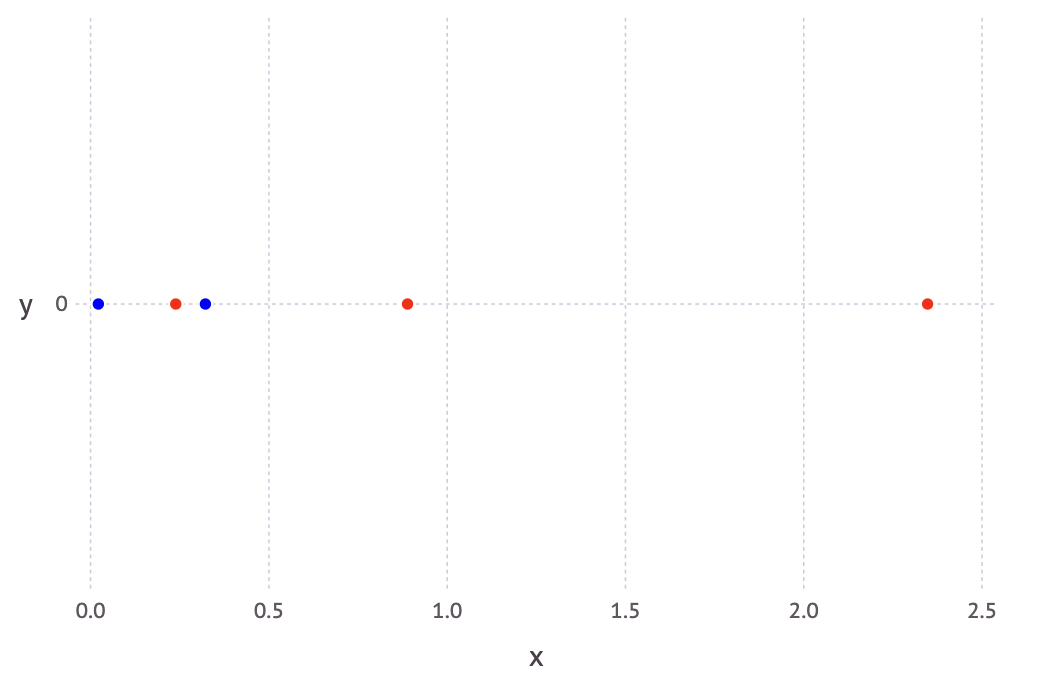
\includegraphics[width=0.7\textwidth]{plot.png}
    \caption{Example Plot.}\label{fig:ex_plot}
\end{figure}

The code plots 1 dot at every arrival time (the x-axis represents the time axis), using different colors to indicate different processes.  Your plot should show points (which represent block arrivals) at corresponding positions in time.


\begin{enumerate}[label=(\alph*)]
    \item Simulate and plot one Poisson point process with rate 1/4 for a period of 100 units of time starting from time 0.  We suggest you do this by first generating some independent exponentially distributed (what's its parameter?) inter-arrival times.  Each arrival should be represented by a red dot on the time axis.  You can use any language you like, submit both your code and the plot.
    \paragraph{My Answer:} The parameter of the exponential distribution for the inter-arrival times is \( \lambda = 1/4 \) since the rate of the Poisson point process is 1/4. The following Julia code simulates the Poisson point process (note that \texttt{Exponential} function from \texttt{Distributions} package uses \href{https://juliastats.org/Distributions.jl/stable/univariate/#Distributions.Exponential}{a form} of \( f(\theta, x) = \frac 1 \theta e^{-\frac x \theta} \), hence corresponding to \(\theta = 4 \)) and plots the arrivals as red dots on the time axis in \Cref{fig:arrival_times}.
    \item Simulate a second Poisson point process with a rate 3/4 which is independent of the one in part (a) on the same time axis.  Plot the arrivals as dots using a different color in the same graph.  The two processes are good models for blocks mined by honest miners and blocks mined by an adversary.  It suffices to turn in one graph for parts (a) and (b).
    \paragraph{My Answer:} The parameter of the exponential distribution for the inter-arrival times is \( \lambda = 3/4 \) since the rate of the Poisson point process is 3/4. The following Julia code simulates the second Poisson point process and plots the arrivals as blue dots on the time axis.
    The plot for both parts (a) and (b) is shown in \Cref{fig:arrival_times}.
    \begin{figure}[h!]
        \centering
        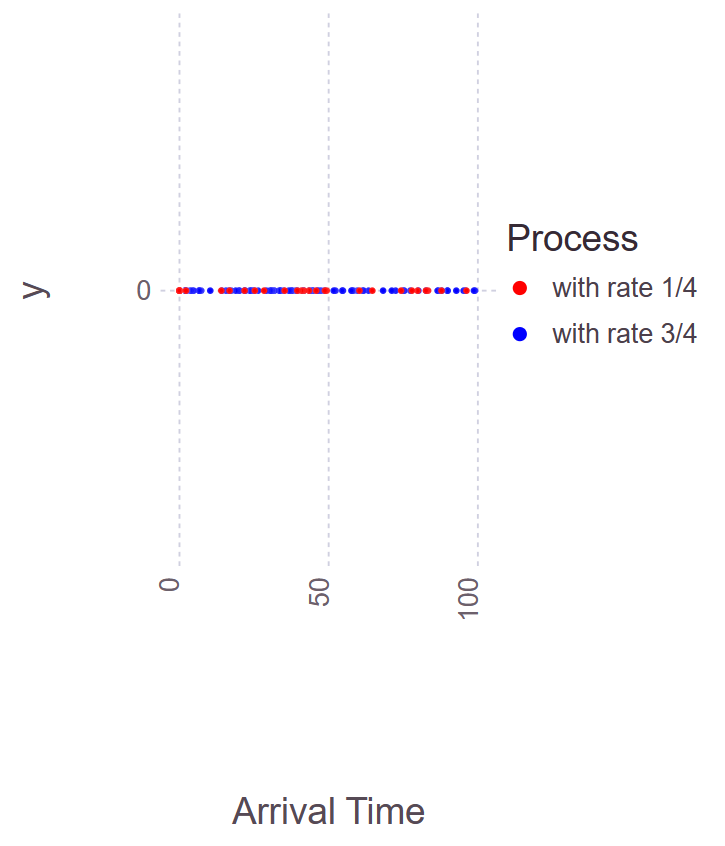
\includegraphics[width=0.7\textwidth]{arrival_times.png}
        \caption{Arrival Times of Poisson Point Processes with Rates 1/4 and 3/4.}\label{fig:arrival_times}
    \end{figure}
    
    The code for both parts (a) and (b) is as follows:
    \begin{lstlisting}[language=Julia, gobble=8]
        using Distributions
        using Gadfly
        using Cairo
        using Fontconfig
        using Colors
        # Generate 100 with rate lambda = 1/4 (theta = 4) as inter-arrival times for at least 
        # 25 samples (n > 25) approximated by 100 time units multiplied by rate (1/4 samples per time unit)
        sample = rand(Exponential(4), 35)
        
        
        # Generate arrival times vector (arrival) from previous inter-arrival times vector (intarrival)
        size = length(sample)
        arrival = zeros(size)
        arrival[1] = sample[1]
        for i in 2:size
            t = sample[i] + arrival[i-1]
            println(t)
            if t > 100  # Stop when the arrival time exceeds 100
                println("break")
                break
            else
                arrival[i] = t
            end
        end
        
        # Generate 100 with rate lambda = 3/4 (theta = 4/3) as inter-arrival times for 
        # at least 75 samples (n > 75) approximated by 100 time units multiplied by rate
        # (3/4 samples per time unit)
        sample2 = rand(Exponential(4/3), 90)
        size2 = length(sample2)
        arrival2 = zeros(size2)
        arrival2[1] = sample2[1]
        for i in 2:size2
            t2 = sample2[i] + arrival2[i-1]
            println(t2)
            if t2 > 100  # Stop when the arrival time exceeds 100
                println("break")
                break
            else
                arrival2[i] = t2
            end
        end
        
        
        # Plot the arrival times as red dots
        yaxis = zeros(length(arrival))
        yaxis2 = zeros(length(arrival2))
        p = Gadfly.plot(layer(x=arrival, y=yaxis, color=[RGBA(1,0,0,0.1)], Geom.point, Theme(point_size=1pt)),
            layer(x=arrival2, y=yaxis2, color=[RGBA(0,0,1,0.1)], Geom.point, Theme(point_size=1pt)),
            Guide.xlabel("Arrival Time"),
            Guide.manual_color_key("Process", ["with rate 1/4", "with rate 3/4"], ["red", "blue"])
            )
        display(p)
    \end{lstlisting}
    \item Use the following different method to produce two mining processes.  First simulate a Poisson point process with rate 1 on the time interval $(0,100]$\@.  For each dot, plot it using one color with probability 1/4 and the other color with probability 3/4, independent of other dots/arrivals.
    \paragraph{My Answer} The following Julia code simulates the Poisson point process:

    \begin{lstlisting}[language=Julia, gobble=8]
        using Distributions
        using Gadfly
        using Cairo
        using Fontconfig
        using Colors
        # Generate 100 with rate lambda = 1 as inter-arrival times for at least 100 samples (n > 100) approximated by 100 time units multiplied by rate (1 samples per time unit)
        sample = rand(Exponential(1), 100)
        
        # Generate arrival times vector (arrival) from previous inter-arrival times vector (intarrival)
        size = length(sample)
        arrival = zeros(size)
        arrival[1] = sample[1]
        for i in 2:size
            t = sample[i] + arrival[i-1]
            println(t)
            if t > 100  # Stop when the arrival time exceeds 100
                println("break")
                break
            else
                arrival[i] = t
            end
        end
        
        # Generate random colors for each arrival
        colors = [rand() < 0.25 ? RGBA(1,0,0,0.1) : RGBA(0,0,1,0.1) for i in 1:length(arrival)]
        
        # Plot the arrival times with random colors
        yaxis = zeros(length(arrival))
        p = Gadfly.plot(layer(x=arrival, y=yaxis, color=colors, Geom.point, Theme(point_size=1pt)),
            Guide.xlabel("Arrival Time"),
            Guide.manual_color_key("Process", ["with rate 1"], ["red", "blue"])
            )
        display(p)
    \end{lstlisting}
    The plot for the mining processes is shown in \Cref{fig:arrival_times2}.
    \begin{figure}[h!]
        \centering
        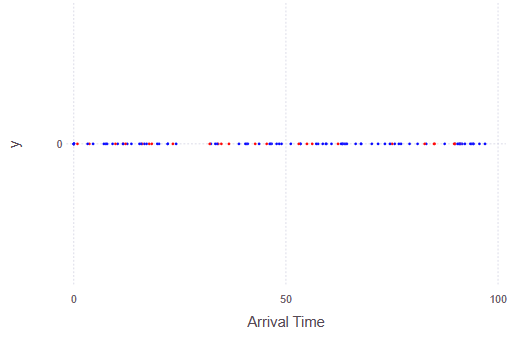
\includegraphics[width=0.7\textwidth]{arrival_times2.png}
        \caption{Arrival Times of Poisson Point Process with Rate 1.}\label{fig:arrival_times2}
    \end{figure}
    \item In terms of the statistics of the processes, are the ones produced in (a) and (b) different than the ones produced in (c)?
    \paragraph{My Answer:} If you look at the expected number of the number of arrivals in a given time interval, that of the combination of (a) and (b) are the same as of (c) process. That is, the expected number of arrivals for blue dots and for red dots in a given time interval, 100 units of time, for both cases is all 75 and 25, respectively, which is calculated as the product of the rate and the time interval (given by $\lambda$). Furthermore, the variance of number of arrivals from process (a) along with (b) is \(Var[A] = 75\) for (a) and \(Var[B] = 25\) for (b) (i.e., $\lambda$ according to the row of \textbf{Poisson distribution} of \Cref{tab:prob_distributions}), and the variance of the total number is \(Var[A + B] = Var[A] + Var[B] + Covar[A, B] = Var[A] + Var[B] = 75 + 25 = 100  \). The same also goes to the process (c). For the number of blue points and red points, the variance is \(Var[C_{\text{blue}}] = 75\) and \(Var[C_{\text{red}}] = 25\) according to the \textbf{Binomial distribution} row of \Cref{tab:prob_distributions}, where the variance is calculated as \(np\). In addition, the variance of the total number is \(Var[C_{\text{blue}} + C_{\text{red}}] = Var[C_{\text{blue}}] + Var[C_{\text{red}}] = 75 + 25 = 100\). Therefore, the statistics of the processes produced in (a) and (b) are the same as the ones produced in (c).
\end{enumerate}

\section{Probability Analysis}
Suppose the proof-of-work mining powers in a network is such that 3/4 of the total power is honest and 1/4 is adversarial.  What is the probability that the adversary mines five or more of the first ten blocks?  [Hint: Think of the model in Problem 3(c).  Consider to use the binomial distribution.]
\paragraph{My Answer:}
The probability can be calculated using the binomial distribution. Let \( X \) be the number of blocks mined by the adversary in the first ten blocks.  Then, \( X \) follows a binomial distribution with parameters \( n = 10 \) and \( p = 1/4 \). The probability mass function of the binomial distribution is given by
\begin{equation}
    P(n, X=k, p) = \binom{n}{k} p^k (1-p)^{n-k}.
\end{equation}

Hence, The probability that the adversary mines five or more of the first ten blocks is given by
\begin{equation}
    \begin{aligned}
    P(X \geq 5) = & 1 - P(X < 5) \\
                = & 1 - \sum_{k=0}^{4} \binom{10}{k} \left(\frac{1}{4}\right)^k \left(\frac{3}{4}\right)^{10-k} \\
                = & 0.07812690734863281.
    \end{aligned}
\end{equation}

\section{Memoryless Property of Poisson Processes}
A Poisson point process with rate h satisfies the following:  The number of blocks mined during period $(s,s+t]$ with $s,t > 0$ is a Poisson random variable with mean ht (the product of h and t).
\begin{enumerate}[label=(\alph*)]
    \item Let $s,t>0$ be real numbers. Calculate
          \[ P\left(\text{the } (k+1)\text{-st block is mined after time } s+t \bigm| \text{the } k\text{-th block is mined by time } s\right). \]
    \paragraph{My Answer:} The probability that the \((k+1)\)-st block is mined after time \( s+t \) given that the \( k \)-th block is mined by time \( s \) is the same as no block being mined in the time interval \((s,s+t]\), which is described by the poisson distribution with rate \( h \).  The probability is given by

    \begin{equation} 
        P(\text{no block is mined in } (s,s+t]) = \frac {e^{-h(s+t-s)} (h(s+t-s))^0} {0!} = e^{-ht}.
    \end{equation}\label{eq:prob_no_block}

    \item What is the distribution of the time between the \(k\)-th block's mining time and the \((k+1)\)-st block's mining time? [Hint: Use the result of (a).]
    \paragraph{My Answer:} Since we have the probability that the \((k+1)\)-st block is mined after time \( s+t \) given that the \( k \)-th block is mined by time \( s \), that also means the probabilty that the \((k+1)\)-st block is mined \textbf{before} time \( s+t \) given that the \( k \)-th block is mined by time \( s \) is \( P(s \leq T \leq s+t) = 1 - e^{-ht} \), which is the cumulative distribution function (CDF).  We can then obtain the distribution of the time between the \( k \)-th block's mining time and the \((k+1)\)-st block's mining time by taking the derivative of CDF to get the probability density function (PDF).  The PDF is given by

    \begin{equation}
        f(t) = \frac{d}{dt} (1 - e^{-ht}) = h e^{-ht}.
    \end{equation}

    Note that this proves that the probability distribution of the time between the \( k \)-th block's mining time and the \((k+1)\)-st block's mining time is the same as the distribution of the time between the first and second block's mining time, which is exponential with rate \( h \). This indicates that the Poisson process is memoryless.

\end{enumerate}

\end{document}
